%This section contains work progress
%In this section is described work progress in each iteration.
This section provides details of the work progress in each iteration
\comment[Petr]{Tam}{Approved? The whole section need to revised again (and again)}

\subsection{Initialization}
TextAn team visited policeman plk. Ing. Jan Hořínek, who introduced us his work and showed
%us existing inadequate software whose extension we should prepare. Basis of the
us the existing inadequate software. We were given the task of preparing an extension. Basis of the
project was to police reports - recognize entities and match them
to existing objects in the database. We were advised to use Webservices for an easy integration of 
the project to the current system. He promised us models and
example data inputs and expected outputs. We divided the work as follows:

\begin{itemize}
\item \textbf{Petr Fanta} - entities recognition and input parsing, look for useful existing solutions
\item \textbf{Adam Huječek} - GUI validation, component schema and communication
\item \textbf{Václav Pernička} - database
\item \textbf{Peter Šípoš} - left the project before it started
\item \textbf{Jakub Vlček} - entities recognition and input parsing, look for useful existing solutions
\end{itemize}


We made some decisions and requirements for each component:

\paragraph{Database}
\comment[anyone]{Jakub}{has anyone better image?}
At the beginning, we made database schema~\ref{fig:dbpilot}, which was approved \comment{Venca}{improved?} after a few
iterations. The main attention was paid on schema generality because we want to
support more than one domain (not just police report).\\
Database should support versioning, parallel processing and partial records. We
decided to create special layer between server and database because of
generality (it will be easier to change database system). Logging (users,
changes) support is also required. It would be a problem merging two objects into 
one, so we created special functionality and table in the
database.
\begin{figure}[!htb]
        \centering
        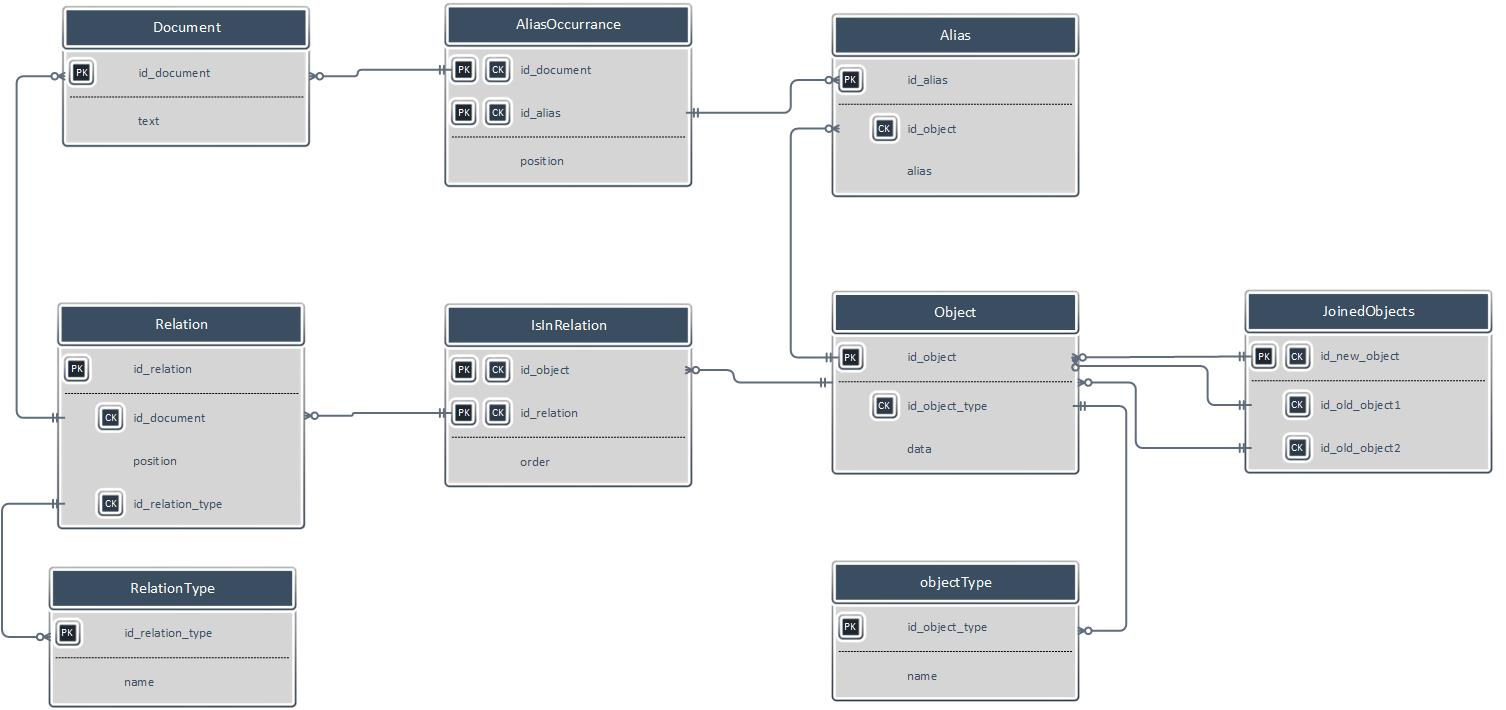
\includegraphics[width=\textwidth]{Images/db-pilot}
        \caption{Pilot database schema.}
        \label{fig:dbpilot}
\end{figure}
\comment[Petr]{Tam}{Need to revised again}

\paragraph{Client}
We decided to use pipeline model. %This means that report processing will consist of more successive phases:
In other words, the report processing consists of several phrases:

\begin{enumerate}
\item Report insertion
\item Report editing
\item (Auto) Entity recognition
\item Entity editing (entity types, ranges, creating new ones)
\item (Auto) Object recognition
\item Object editing (adding new ones, repair bad connections between entities and objects)
\item (Auto) Relationships recognition
\item Relationships editing
\item Report confirmed and sent to server
\end{enumerate}

Changes in each phase are not stored in the database immediately but
stored locally. They would be written to database after confirmation. There was problem with
machine recognition, because models with newly added items are trained after final 
confirmation, so it is impractical to learn from the output. 
We decided, that newly added items will be preferred over recognized ones
\comment[Petr]{Tam}{Need to revised again} 
 
\subsection{Design \& technologies}
In November, we mainly chose and tested technologies which we could use. New member Duc Tam Hoang joined \textan{},. His specialization is
linguistic and machine learning so he will be really useful for our project.
Because of Tam's limitation in Czech, the document language was changed to English.
His main task will be NER and entity-object matching. We were trying different
entity recognizers, but there are not many applicable for Czech. Milan Straka
promised us his project NameTag. It is named entity recognizer for Czech, so
exactly what we need. Problem is, that it is not finished yet and in C++
language, so there must be additional layer between Java and C++.
We researched possibilities about entity-object matching. Program will get
entity and assign it possible candidates from objects. This part could not be
purely automatic because of ambiguity, but if there will be high probability,
program should match object entity pair automatically.

Possible solutions for entity-object matching are machine learning  methods
ranking or classification.

We looked for suitable Java library which provides machine learning techniques.
Candidates were JavaML and Weka. We have tested them and at first, we chose
JavaML, because it provides more machine learning algorithms (some of them uses
WEKA library) and because of WEKA problem - WEKA  was created for teaching purposes so
it's performance is not as good as JavaML.
Than we found, that we don't need these functions and because JavaML seems no longer be supported and that
new version of WEKA was released, so we choose WEKA, because it's a live project and its functionality is enough for us.

There were two possible server architectures: standalone or embedded webserver
(Tomcat or Jetty). We considered usage of some technologies like Spring, CXF and
Hibernate for database layer.

\subsection{Prototyping \& interconnecting}
After the technologies were chosen, we made some prototypes of each component. We
discussed a lot of APIs (we need them for testing). For testing purposes, we must
provide some mock objects, so everyone implemented mock of his component.
NameTag was released, so we tried to get acquaintance. We met Milan Straka, the author of NameTag.
He presented and helped us get familiar with NameTag. We started stared testing it.
There were problems with compiling and Java bindings, which took more time than we expected. Problem was missing documentation.
We connected client and database to server, implemented database data browsing on client (mainly graphs viewing with JUNG).
Tam made prototype of object matcher, but it was not integrated to server.

\subsection{Main coding}
When we made a prototype of whole program, everyone started improving his component in his own branch.
\paragraph{Server} Server was debugged and made reliable. It starts using WSDLs so there were lot of work on server and client parts. Result was, that Java code is now generated automatically. Connection to database was reworked to use Spring Beans.
\paragraph{Named entity recognizer} NameTag was fully integrated to server. We started editing it for our purposes (using our structures and types). There were problems with gazetteers files and translating entities from NameTag to Textan.
After receiving information that NameTag will not support JNI to training parts, we researching how to launch training binaries from Java.
\paragraph{Client} Client was reworked to pipeline as we need, we improved graph viewing to support oriented edges.
\paragraph{Object matcher} TextPro (as we called entity-object matching) has first prototype. It uses a simple ranking method, which resulted in a poor performance. 
\paragraph{Database} Database has new layer with DAOs, so no more need to access database directly.
After this iteration, we released first alpha version of TextAn.

\subsection{Improving}
Alpha version of NameTag learning was implemented. There were few problems with portability because of different architectures and operating systems. After implementing special functions in database, we made automatic data extraction for learning. For this purpose, new function to server was added - commands. It is the implementation of design pattern Command, which started data generation and model training after new report insertion. Models managing implemented due to bigger size (deleting old ones) 
Database support logging. It was done through interceptors - triggers in Hibernate layer.
In client, there were lots of small fixes in GUI, problems were with portability between Windows and Unix-like systems, where ControlsFX and JavaFX behave differently.
TextPro received many new features. We integrated Morphodita because we needed its tagger for new features.
Settings through properties files are now supported in each component.

\subsection{Bugfixing \& documentation}
For final testing, we created server hosted by university with address Ttextan.ms.mff.cuni.cz. Here we always have the newest version from master branch.
